\documentclass[letterpaper,12pt]{article}

\oddsidemargin 0.0in
\topmargin 0.25in
\headheight 0.0in
\headsep 0.25in
\evensidemargin 0.0in
\textwidth 6.5in
\textheight 8in

\usepackage{color}
\usepackage{textcomp}
\usepackage{listings}
\lstset{
  tabsize=2,
  language=ruby,
  morecomment=[l]{//},
  basicstyle=\scriptsize,
  columns=fixed,
  breaklines=true,
  extendedchars=true,
  showspaces=false,
  showstringspaces=true,
}

\usepackage{hyperref}

\usepackage{graphics}

\author{Will Farrington, Jeff Drasher, Mike Hirth}
\title{Calculus 3 for Computer Science Project}

\begin{document}

\maketitle
\tableofcontents
\newpage
\section{Introduction}

Much of the code used within this assignment is Ruby version 1.9.x.
Since it is, for most intents and purposes, a lesser known language than say,
Java, we felt it necessary to explain bits of the language which might surface
in the code we wrote for this project.

\subsection{Ruby}

First and foremost, Ruby shares many similarites with, and is inspired by, Lisp,
Smalltalk, and Perl (most likely in that order).
It contains many of the niceties of functional programming that Lisp does, it is
truly object oriented in the same way Smalltalk is, and it is a terse scripting
language with powerful features like Perl is.

\subsubsection{Syntax, Language Quirks, Etc.}

Notations that might seem confusing unless one has a background in all three of
these languages are such:

\begin{description}

\item[Basic Syntax]

  Comments are preceded by a \texttt{\#}.
  Strings are wrapped in either single- or double-quotes.
  Indentation is two spaces.
  Rather than using indentation-based block delimiters or curly braces,
  Ruby simply uses the end keyword.

\item[Blocks]

  Blocks are notations for anonymous functions in Ruby (like lambda in Lisp).
  They can be written a number of ways, such as:
  
  \begin{lstlisting}[language=ruby]
    # Assigning a lambda/proc to a variable, and then calling it
    f = ->(x){ x + 1 }
    f[2] #=> 3

    # Array#map is one of several functions which takes a block as an argument
    a = [1,2,3]
    a.map { |i| i * i } #=> [1,4,9]

    # This is the expanded form of the block, used for creating multi-line anonymous functions
    a.each do |item|
      puts item
    end
    # would print 1, 2, and 3 on separate lines
  \end{lstlisting}
  
\item[Ranges]
  
  Ranges are represented in Ruby with one of two operators, \texttt{..} or \texttt{...}.
  \texttt{0..10} is an inclusive range ($[0,10]$) in a more mathematical notation,
  whereas \texttt{0...5} is exclusive ($[0,5)$).
  Ranges can be iterated across.
  
\item[Method Invocation]

  In Ruby, method invocation has optional parens.
  Rather than using the form \texttt{instance.method(arg1, arg2)},
  one can use the form \texttt{instance.method arg1, arg2}.
  In the case where an invocation doesn't have arguments,
  the parentheses are still optional.

\item[Object Oriented]

  Ruby, like Smalltalk, is object oriented down to the primitives of the language.
  This means that all things in Ruby are objects, and thus have methods that can
  operate on them.
  This library was written to make use of this, monkey-patching functionality into
  the existing Matrix and Vector classes in Ruby.

\item[Notation]

  Ruby has a common nomenclature for expressing its classes and their methods.
  \texttt{Object\#method} is the de facto standard among Rubyists, hence, that's the form
  we'll use here.
  Similarly, \texttt{\#=$>$} is used to denote return values.

\item[Further Notes]

  Ruby's Matrix and Vector classes lack \texttt{\#[]=} methods, therefore, we often convert
  these two datatypes to arrays and back again to perform matrix or vector arithmetic
  or other operations.

\end{description}

Hopefully, that should clear up any misconceptions or confusion before
addressing the actual code at hand.
That said, all three parts of this report do make use of both some standard
libraries in Ruby, as well as extensions upon them.

\begin{itemize}

\item \texttt{http://www.ruby-doc.org/core/classes/Array.html}
\item \texttt{http://www.ruby-doc.org/core/classes/Matrix.html}
\item \texttt{http://www.ruby-doc.org/core/classes/Vector.html}

\end{itemize}

\subsubsection{Common Code}

Additionally, we wrote an abstraction layer into some of these classes via
monkeypatching in order to add some common functionality:

\lstset{caption=Common Code for All Three Parts}
\begin{lstlisting}[language=ruby]
class Vector
  private
  def sign(x)
    return 1 if x > 0
    return -1 if x < 0
    return 0
  end
end

class Matrix
  def pretty_print
    str = ""
    self.to_a.each do |row|
      row.each do |i|
        if i.to_i >= 0
          str << " "
        end
        if ("%.3f" % i).to_f == i.to_i
          str << "#{i.to_i}     "
        else
          str << "%.3f " % i
        end
      end
      str << "\n"
    end
    puts str
  end

  def inf_norm
    self.to_a.map do |a|
      a.map do |ar|
        ar.abs
      end.inject(&:+)
    end.sort[0]
  end

  def is_lower_triangular?
    triangular(self.column_vectors)
  end

  def is_upper_triangular?
    triangular(self.row_vectors)
  end

  private
  def triangular(vecs)
    for i in 0...vecs.length
      vec = vecs[i].to_a
      unless i <= 1
        return false unless vec[0...i].all? { |n| n == 0 } and vec[i..-1].all? { |n| n != 0 }
      end
    end
    return true
  end
end
\end{lstlisting}

\subsection{Java}

Part Two is written in Java.
The code therein extends the Matrix class with a few methods and constructors.
We assume that Java's syntax is understood by the reader given its prominence,
especially here at Georgia Tech.

\subsection{About This Document}

This document was typeset in \LaTeX.
It uses the \textit{color} and \textit{listings} packages for the code
formatting.
It additionally uses \textit{hyperref} for in-document links in the compiled PDF.

The source code for this document is available, along with the compiled PDF form, at
\texttt{http://github.com/wfarr/calc3-for-cs/blob/master/report/report.tex}.
All of the actual code used in the report, along with data output from the code
can be viewed at \texttt{http://github.com/wfarr/calc3-for-cs/tree/master/code}.
The unique advantage of viewing the code this way is that the user can walk
through individual commits and see the code evolve into its final form (the
same can be said of the report, since it is in fact just code and content).

\newpage
\section{Part One}

%%
%% By: Will Farrington
%%

The purpose of Part One of the project is to solve the typical
$A\vec{x} = \vec{b}$ equation, with $A$ being a Hilbert matrix.
A Hilbert matrix is a square matrix whose elements follow the form

\[H_{ij} = \frac{1}{i + j - 1}\]

Here's an implementation in Ruby:

\lstset{caption=Hilbert Matrix Implementation}
\begin{lstlisting}[language=ruby]
class Matrix
  def self.hilbert(n)
    m = Matrix.zero(n).to_a
    m = m.each_index.map{|row| m[row].each_index.map{|col| 1 / (row + col + 1)}}
    return Matrix.rows(m)
  end
end

Matrix.hilbert(4) #=> Matrix[[1/1,1/2,1/3,1/4], [1/2,1/3,1/4,1/5], [1/3,1/4,1/5,1/6], [1/4,1/5,1/6,1/7]]
\end{lstlisting}

Often times, simplifying a single matrix $A$ into two or more ``nicer'' matrices
(in the case of these algorithms, $LU$ or $QR$) can make solving the equation
$A\vec{x}=\vec{b}$ easier.
Such algorithms introduce the potential for error, namely because they are
modified forms of the original matrix.

\subsection{LU Decomposition}

LU Decomposition uses matrix multiplication to reduce a matrix $A$ into two
matrices, $L$ (a lower triangular matrix) and $U$ (an upper triangular matrix).

\subsubsection{Explanation of the Algorithm}

The algorithm for doing so is fairly simple in and of itself:

\begin{enumerate}
\item Starting with the first column, find the first non-zero entry below the
  diagonal. Let this entry be considered $x$. Let that column's diagonal element
  be $y$.
\item Multiply an Identity matrix, with the location of the entry $x$ set to the
  value $-\frac{x}{y}$. This matrix is $L_n$.
\item The resulting matrix is the new $A$ for the next iteration.
\item Repeat these steps until the resulting $A$ is upper triangular.
  At this point, $A$ becomes $U$.
\item To find $L$, multiply $L_1^{-1}L_2^{-1} ... L_n^{-1}$.
\item Substitute $A$ with $LU$ in the equation $A\vec{x}=\vec{b}$ and solve.
\end{enumerate}

This is commonly known as the Doolittle algorithm.

\subsubsection{Implementation of the Algorithm}

\lstset{caption=LU Decomposition}
\begin{lstlisting}[language=ruby]
class Matrix
  def lu_decomposition
    return nil unless self.square?
    n = self.row_size
    a = self
    l_n = []
    cvs = a.column_vectors.map { |v| v.to_a }
    for k in 0...cvs.length
      for j in 0...cvs.length
        l_new = Matrix.identity(n).to_a
        if l_new[j][k] == 1 || j < k
          next
        end
        l_new[j][k] = - (cvs[k][j] / cvs[k][k])
        l_n << l_new
        a = Matrix[*l_new] * Matrix[*cvs.transpose]
        cvs = a.column_vectors.map { |v| v.to_a }
      end
    end
    l_final = l_n.map { |m| Matrix[*m].inverse }.inject(&:*)
    u_final = a
    return l_final,u_final
  end
end
\end{lstlisting}

The algorithm first begins with an essential check: the method
\texttt{self.square?} determines if the matrix is a square matrix, and returns
true if it is.
LU Decomposition can only be done on square matrices, thus, the method returns
nil when given a non-square matrix.
Next, the algorithm defines $A$ (written as \texttt{a} in the code because
\texttt{A} would've been a Constant rather than a variable) to be the instance
of \texttt{self}.
To iterate across the columns efficiently, we use
\texttt{Matrix\#column\_vectors}, which returns an array of column vectors.
This array is then \texttt{map}ped over to convert the vectors into arrays.
The end result is that \texttt{cvs} is an array of arrays representing the
columns of \texttt{self}.

The actual computation lies in the nested \texttt{for} loops.
For each iteration, an \texttt{l\_new} matrix is created and converted to an
array.
If the current values of \texttt{j} and \texttt{k} are above the diagonal,
then the algorithm skips to the next iteration.
Next, \texttt{l\_new[j][k]} is set to $-\frac{x}{y}$, as above in the
algorithm's description.
A new \texttt{a} is made as the product of \texttt{l\_new} and
\texttt{cvs.transpose} (the same matrix as $A$).
The last step of each iteration is rebuilding \texttt{cvs} based off of the
newest \texttt{a}.

Finally, $L$ and $U$ are assigned and returned.
While \texttt{u\_final} is straight-forward, \texttt{l\_final} is a bit more
complicated.
\texttt{l\_n.map \{ |m| Matrix[*m].inverse \}} returns an array of inverted
matrices from the original array of arrays (of arrays).
The one bit of syntactic sugar in that line is the use of \texttt{Matrix[*m]}.
In this case, \texttt{*} is acting as the glob operator, essentially inserting
all the content of the array it's called on rather than simply inserting the
array itself.

This is necessary because \texttt{Matrix[...]} takes a list of rows (in the
form of arrays) as its argument.
Finally, this new array is passed \texttt{Array\#inject}, which applies a given
block to all elements of an array and returns the result.
In this case, the injection is making use of a feature in Ruby 1.9 called
\texttt{symbol\_to\_proc}, which allows for passing the method the \texttt{:*}
symbol and automatically converting it into a proc/lambda.
Thus, the result of the injection is to multiply all the results of the map
together, in order.
\\
\subsubsection{Results and Analysis}

Below are the results from the solving $LU\vec{x} = \vec{b}$ for $\vec{x}$.
\texttt{sol} is the solution vector.
Errors are not listed for these computations because the resulting errors are
all 0.
This is because the LU algorithm used here doesn't introduce any additional
error.
However, there is still technically error inherent in the problem itself,
which can be found by evaluating $cond{(LU)}$ because $cond(A) = cond(LU) \le cond(L) cond(U)$.

\begin{quote}
N = 2
\\sol = Vector[-2, 6]
\\
\\N = 3
\\sol = Vector[3, -24, 30]
\\
\\N = 4
\\sol = Vector[-4, 60, -180, 140]
\\
\\N = 5
\\sol = Vector[5, -120, 630, -1120, 630]
\\
\\N = 6
\\sol = Vector[-6, 210, -1680, 5040, -6300, 2772]
\\
\\N = 7
\\sol = Vector[7, -336, 3780, -16800, 34650, -33264, 12012]
\\
\\N = 8
\\sol = Vector[-8, 504, -7560, 46200, -138600, 216216, -168168, 51480]
\\
\\N = 9
\\sol = Vector[9, -720, 13860, -110880, 450450, -1009008, 1261260, -823680, 218790]
\\
\\N = 10
\\sol = Vector[-10, 990, -23760, 240240, -1261260, 3783780, -6726720, 7001280, -3938220, 923780]
\\
\\N = 11
\\sol = Vector[11, -1320, 38610, -480480, 3153150, -12108096, 28588560, -42007680, 37413090, -18475600, 3879876]
\\
\\N = 12
\\sol = Vector[-12, 1716, -60060, 900900, -7207200, 34306272, -102918816, 199536480, -249420600, 193993800, -85357272, 16224936]
\\
\\N = 13
\\sol = Vector[13, -2184, 90090, -1601600, 15315300, -88216128, 325909584, -798145920, 1309458150, -1422621200, 981608628, -389398464, 67603900]
\\
\\N = 14
\\sol = Vector[-14, 2730, -131040, 2722720, -30630600, 209513304, -931170240, 2793510720, -5761615860, 8180071900, -7852869024, 4867480800, -1757701400, 280816200]
\\
\\N = 15
\\sol = Vector[15, -3360, 185640, -4455360, 58198140, -465585120, 2444321880, -8779605120, 22086194130, -39264345120, 49080431400, -42184833600, 23728968900, -7862853600, 1163381400]
\\
\\N = 16
\\sol = Vector[-16, 4080, -257040, 7054320, -105814800, 977728752, -5975009040, 25241364720, -75724094160, 163601438000, -255218243280, 284747626800, -221470376400, 114011377200, -34901442000, 4808643120]
\\
\\N = 17
\\sol = Vector[17, -4896, 348840, -10852800, 185175900, -1955457504, 13742520792, -67310305920, 236637794250, -607662484000, 1148482094760, -1594586710080, 1605660228900, -1140113772000, 540972351000, -153876579840, 19835652870]
\\
\\N = 18
\\sol = Vector[-18, 5814, -465120, 16279200, -313374600, 3747960216, -29983681728, 168275764800, -683620294500, 2050860883500, -4593928379040, 7707169098720, -9633961373400, 8835881733000, -5770371744000, 2538963567360, -674412197580, 81676217700]
\\
\\N = 19
\\sol = Vector[19, -6840, 610470, -23876160, 514829700, -6919311168, 62466003600, -397742716800, 1845774795150, -6380456082000, 16652990374020, -33030724708800, 49775467095900, -56549643091200, 47605566888000, -28774920430080, 11802213457650, -2940343837200, 335780006100]
\\
\\N = 20
\\sol = Vector[-20, 7980, -790020, 34321980, -823727520, 12355912800, -124932007200, 894921112800, -4698335842200, 18503322637800, -55509967913400, 127994058246600, -227544992438400, 311023037001600, -323717854838400, 251780553763200, -141626561491800, 54396360988200, -12759640231800, 1378465288200]
\end{quote}


\begin{figure}[h] 
  \centering
  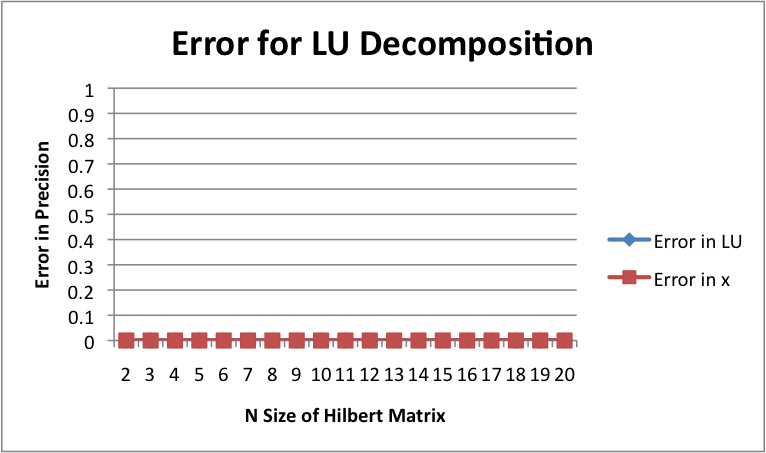
\includegraphics{LU.png}
  \caption{\label{LU}Error for LU Decomposition.}
\end{figure}


\subsection{Householder Reflections}

The Householder Reflection is, as Wikipedia might say: ``a linear transformation
that describes a reflection in a hyperplane (containing the origin)''.

\subsubsection{Description of the Algorithm}

\begin{enumerate}
\item Let $\vec{a}$ be the first column of the given matrix $A$.
\item Let $\vec{u} = (a_1 + sign(a_1) * ||\vec{a}||, a_2, a_3, ..., a_n)^t$.
\item Let \[H(\vec{a}) = I - 2 \frac{\vec{u}\vec{u}^t}{||\vec{u}||^2}\]
\item If $H(\vec{a})$ is the same size as $A$, $H(\vec{a}) = H_1$.
  Else, let $H_1$ be an Identity matrix, where the bottom right $n \times n$
  entries are the contents of $H(\vec{a})$.
\item Let $A_1 = H_1 A$.
\item Let $\vec{a2}$ be the second column of $A_1$, using only the items including
  and below the diagonal.
\item Let $\vec{u2} = (a2_1 + sign(a2_1) * ||\vec{a2}||, a2_2, a2_3, ..., a2_n)^t$.
\item Find $H(\vec{a2})$ as described above.
\item Find $H_2$ as described above.
\item Let $A_2 = H_2 A_1$.
\item Repeat the above as necessary until $A_n$ is upper triangular. $A_n = R$.
\item $Q = H_1 H_2 H_{(n-1)} H_n$.
\end{enumerate}

\subsubsection{Implementation of the Algorithm}

\lstset{caption=QR Decomposition via Householder Reflections}
\begin{lstlisting}[language=ruby]
class Matrix
  def householder
    return nil unless self.square?
    current_iteration = self
    init_dim = self.row_size
    h_list = []
    cv = current_iteration.column_vectors[0]
    h = (cv.find_householder_reflection - Matrix.identity(cv.size)).expand_to_dimensions(init_dim,init_dim) + Matrix.identity(init_dim)
    h_list << h
    current_iteration = h * current_iteration
    for i in 0...self.row_size
      cv = current_iteration.get_column_vector(i+1)
      break if cv.size < 2 || current_iteration.is_upper_triangular?
      h = (cv.find_householder_reflection - Matrix.identity(cv.size)).expand_to_dimensions(init_dim,init_dim) + Matrix.identity(init_dim)
      h_list << h
      current_iteration = h * current_iteration
    end
    q,r = h_list.inject(&:*), current_iteration
    return q,r
  end

  def expand_to_dimensions(x,y)
    curr_x, curr_y, a = self.row_size, self.column_size, self.to_a
    a.each_index do |row|
      for i in 0...(y - curr_y)
        a[row] = a[row].insert(0,0)
      end
    end
    for i in 0...(x - curr_x)
      a = a.insert(0,Array.new(y){0})
    end
    return Matrix.rows(a)
  end

  def get_column_vector(x)
    return Vector.elements(self.column(x)[x..-1])
  end
end

class Vector
  def find_householder_reflection
    a = self.to_a
    a = a[0] if a[0].is_a?(Array)
    a[0] = a[0] + sign(a[0]) * self.r
    u = Vector[*a]
    norm_u_sqrd = u.r**2
    uut = u.covector.transpose * u.covector
    h = Matrix.identity(uut.row_size) - (uut * (2 / norm_u_sqrd))
    return h
  end
end
\end{lstlisting}

\texttt{Matrix\#householder} begins by asserting that the instance of
\texttt{self} is a square matrix (which, since it ought to be a Hilbert matrix,
it should be).
\texttt{current\_iteration} is assigned to \texttt{self}, for now, but in the
algorithm itself, it is really $A_n$.
\texttt{init\_dim} is $n$ for this $n \times n$ matrix, and is used for
\texttt{Matrix\#expand\_to\_dimensions}, which serves to form an $n \times n$
matrix the same size as \texttt{self}, where $H(\vec{a\textit{n}})$ is the bottom-right
$j \times j$ entries of the matrix and all other entries are 0, for iterations of the Householder
Reflection past the first (as described in step 4).
Because the Householder Reflection works by essentially iterating across the
column vectors of a matrix, we store the current column vector in \texttt{cv}.
\texttt{h} is found by first calling the \texttt{Vector\#find\_householder\_reflection}
method, which takes \texttt{self} (an instance of \texttt{Vector}) and finds $(I - 2\vec{u}\vec{u}^t / ||\vec{u}||^2)$;
then, we subtract an Identity matrix of \texttt{cv.size} from it, so that,
when the matrix is expanded to the right dimensions, we can simply add an
Identity matrix of size \texttt{init\_dim} to it, and thus determine
$H_n$.
\texttt{h} is then appended to \texttt{h\_list}, which stores all given
$H_n$ matrices so $Q$ can be found at the end of the process.
\texttt{current\_iteration} then becomes \texttt{h * current\_iteration},
as it is again $A_n$.
This process is repeated in the \texttt{for} loop until $A_n$ is upper triangular.

Once the \texttt{for} loop is done, \texttt{q} is found by \texttt{inject}ing \texttt{:*}
to the array (finding the product of all its elements), and then the method
returns both \texttt{q} and \texttt{r}.
\\
\subsubsection{Results and Analysis}

Below are the solutions for $n = 2,3,...,20$ and their respective errors.
\texttt{sol} is the solution to the equation $QR\vec{x}=\vec{b}$, \texttt{err1}
is $||QR - H||_{\infty}$ and \texttt{err2} is $||H\vec{x} - \vec{b}||_{\infty}$.
It is important to note that regardless of the other error measurements, there
remains inherent error in the original problem; however, it is more stable than
other decompositions as $Q$ is orthogonal, and its condition number becomes 1,
making $cond(A) = cond(QR) = cond(R)$.

\begin{quote}
N = 2
\\sol = Vector[-2.0, 6.0]
\\err1 = 1.66533453693773e-16
\\err2 = 1.60118641699469e-15
\\
\\N = 3
\\sol = Vector[3.00000000000003, -24.0000000000001, 30.0000000000001]
\\err1 = 1.94289029309402e-16
\\err2 = 1.52807993228568e-14
\\
\\N = 4
\\sol = Vector[-3.99999999999912, 59.9999999999891, -179.999999999973, 139.999999999983]
\\err1 = 8.32667268468867e-17
\\err2 = 9.99822253751169e-14
\\
\\N = 5
\\sol = Vector[5.000000000005, -120.000000000098, 630.000000000437, -1120.0000000007, 630.00000000032]
\\err1 = 2.77555756156289e-17
\\err2 = 1.52010783481848e-11
\\
\\N = 6
\\sol = Vector[-6.00000000089631, 210.000000026659, -1680.00000018463, 5040.00000048848, -6300.00000054552, 2772.00000021677]
\\err1 = 1.66533453693773e-16
\\err2 = 4.50239798778978e-11
\\
\\N = 7
\\sol = Vector[7.00000002203342, -336.000000875792, 3780.00000842381, -16800.000032749, 34650.0000600293, -33264.0000519156, 12012.0000170525]
\\err1 = 5.55111512312578e-17
\\err2 = 1.06241414529746e-08
\\
\\N = 8
\\sol = Vector[-7.99999865279824, 503.999925690703, -7559.99901077151, 46199.9945707619, -138599.985226035, 216215.978917003, -168167.984892845, 51479.9957131147]
\\err1 = 1.52655665885959e-16
\\err2 = 2.09425467726484e-07
\\
\\N = 9
\\sol = Vector[8.99991121736821, -719.993737591431, 13859.8922690749, -110879.221232176, 450447.11486721, -1009002.0608654, 1261253.1328125, -823675.828304291, 218788.96420002]
\\err1 = 1.17961196366423e-16
\\err2 = 1.21468854032131e-06
\\
\\N = 10
\\sol = Vector[-9.9992164587602, 989.931160077453, -23758.5153179169, 240226.370779037, -1261194.48214722, 3783598.73800659, -6726421.01654053, 7000989.76269531, -3938067.03869629, 923746.248901367]
\\err1 = 3.81639164714898e-16
\\err2 = 8.29218156290765e-05
\\
\\N = 11
\\sol = Vector[10.9215391352773, -1311.73552900553, 38394.4682121277, -478059.230010986, 3138670.80151367, -12057010.7783203, 28476986.6474609, -41855156.7421875, 37286086.8505859, -18416710.2607422, 3868220.01245117]
\\err1 = 2.28983498828939e-16
\\err2 = 0.00185948780040064
\\
\\N = 12
\\sol = Vector[-11.6805649157614, 1679.12435483932, -58989.5669555664, 887300.243652344, -7113479.57226562, 33916613.15625, -101885819.21875, 197749121.4375, -247409658.1875, 192575582.5, -84787765.75, 16125571.2402344]
\\err1 = 8.32667268468867e-17
\\err2 = 0.0585635613263169
\\
\\N = 13
\\sol = Vector[-17.629118386656, 2490.83803939819, -86599.147064209, 1297060.88525391, -10418336.40625, 50111503.28125, -153161826.6875, 306042975.75, -401453162.5, 338343685.75, -172737279.125, 46734931.15625, -4675286.6953125]
\\err1 = 2.56739074444567e-16
\\err2 = 1.56440400784855
\\
\\N = 14
\\sol = Vector[11.0518277585506, -1764.99642848969, 68637.5826416016, -1136988.75390625, 9953654.8203125, -51021878.3125, 159625676.25, -299363132.0, 285460295.0, 19638141.5, -388452240.125, 449289740.5625, -231062811.6875, 47002828.21875]
\\err1 = 1.11022302462516e-16
\\err2 = 1.33430942738243
\\
\\N = 15
\\sol = Vector[3.29442912340164, -380.200534820557, 7961.71643066406, 4005.939453125, -1492676.53125, 17134611.625, -93579339.75, 288969014.0, -501815422.0, 360213708.0, 326874200.0, -1012593684.0, 1003466117.0, -480407496.0, 93219587.1875]
\\err1 = 1.52655665885959e-16
\\err2 = 2.91871352864347
\\
\\N = 16
\\sol = Vector[3.48647512495518, -349.450300216675, 5386.19491577148, 54487.87109375, -1854269.609375, 17502754.9375, -84299294.625, 228281192.75, -323287753.5, 95025811.625, 424792122.0, -671701552.0, 339574854.0, 80873993.5, -147689482.0, 42722294.125]
\\err1 = 1.2490009027033e-16
\\err2 = 0.32930532191147
\\
\\N = 17
\\sol = Vector[-3.22108361124992, 728.225301265717, -36159.6916503906, 724344.018554688, -7402839.390625, 43077150.21875, -148688391.75, 295754646.5, -275331067.0, -47381104.0, 241467401.0, 230313529.5, -896512947.0, 851724014.0, -286636087.0, -30766117.5, 29693161.5]
\\err1 = 1.38777878078145e-16
\\err2 = 9.96697505353901
\\
\\N = 18
\\sol = Vector[-13.0393237173557, 2013.47146224976, -75089.7684326172, 1170257.80664062, -9283656.0390625, 39911290.9375, -85617516.25, 27606976.125, 287936783.125, -636646629.0, 483502426.0, -37884332.0, 181593149.0, -677921490.0, 485359060.0, 129016824.0, -273697056.0, 85027202.375]
\\err1 = 1.38777878078145e-16
\\err2 = 8.97655984917988
\\
\\N = 19
\\sol = Vector[-10.575250312686, 1318.33017349243, -38301.4317016602, 435838.275390625, -2257109.34375, 5587472.8125, -14746395.5, 107632294.5, -505401583.0, 1146077540.0, -970212002.0, -862750557.0, 2432907180.0, -1225124416.0, -950342148.0, 820311713.0, 549310000.0, -743750960.5, 212360400.75]
\\err1 = 2.25514051876985e-16
\\err2 = 2.63674345603329
\\
\\N = 20
\\sol = Vector[2.00276151299477, -391.758289337158, 18499.1511230469, -364428.8125, 3674418.6875, -20653072.0625, 65033263.25, -100826814.25, 24646409.0, 77025627.0, 218001766.0, -800348840.0, 587811592.0, 426437661.0, -533096001.0, -313934860.0, 292470652.0, 454225316.5, -534529997.0, 154409446.5]
\\err1 = 1.04083408558608e-16
\\err2 = 1.33007968616477
\end{quote}

\begin{figure}[h]
  \centering
  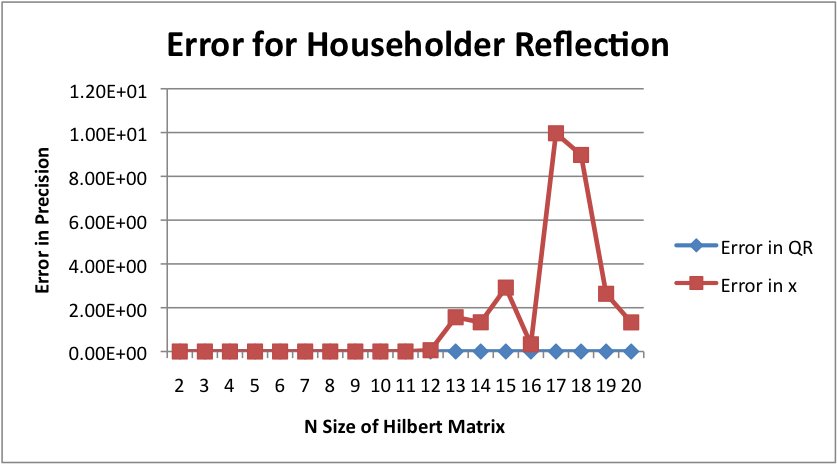
\includegraphics{householder.png}
  \caption{\label{householder}Error for Householder Reflection.}
\end{figure} 


There are a few trends to examine within these results.
First and foremost, it is clear that for the first handful of iterations, the
Householder Reflections are extremely accurate.
However, it is important to note that inaccuracy present at, and the huge
increases in \texttt{err2} after $N =13$.
Since the errors measured above indicated this, but didn't offer any conclusive
reason why (other than error amplification in $\vec{x}$, further investigations
were necessary.
Invoking the same property above, and using the property $||A|| = |\max{\lambda_i}|$,
I used the Power method to find the absolute value of the maximum eigenvalue of
$A$ to compute the $cond(R)$ to determine the inherent error amplification in the
problem.

\lstset{caption=Determining cond(R) for Householder}
\begin{lstlisting}[language=ruby]
for i in 2..20
  m = Matrix.hilbert(i)
  q,r = m.householder
  norm_r = r.power_method.abs
  norm_r_inv = r.inverse.power_method.abs
  puts "cond(N=#{i}): #{norm_r * norm_r_inv}"
end
\end{lstlisting}

As expected, this code snippet printed out condition numbers for each matrix...
up until the 13th iteration.

\begin{quote}
cond(N=2):  15.0000000633676\\
cond(N=3):  299.040132219316\\
cond(N=4):  6349.76484639525\\
cond(N=5):  138457.647018696\\
cond(N=6):  3063599.23761458\\
cond(N=7):  68420347.6630276\\
cond(N=8):  1537937583.62974\\
cond(N=9):  34733563292.8343\\
cond(N=10): 787269502031.433\\
cond(N=11): 17829448576474.5\\
cond(N=12): 4.02515205148727e+14
\end{quote}

Having let the program run for twenty minutes, fully utilizing one 2.4Ghz core
and 8MB RAM, we determined that the solution could not be computed.
This was because the Power Method did not converge to an eigenvalue for
$||R^{-1}||$.
This is most likely because the matrix itself is ill-conditioned, having incredibly
small eigenvalues.
This is more than likely a contributing factor of the inaccuracy of the results
after the 13th iteration.

\subsection{Givens Rotations}

The Givens Rotation, like the Householder Reflection, is a more efficient and
stable decomposition method than Gram-Schmidt.
Unlike the Householder Reflection, however, the Givens Rotation uses counterclockwise
rotations in order to zero out items below the diagonal.
This is done based off of the principle of a standard rotation matrix in 2 dimensions:

\[\left[ \begin{array}{cc} c & s \\ -s & c \end{array} \right]
\left[ \begin{array}{c} a \\ b \end{array} \right] =
\left[ \begin{array}{c} r \\ 0 \end{array} \right] \]

where

\[c = \frac{a_{ii}}{\sqrt{a^2_{ii} + a^2_{ij}}}\]

and

\[s = - \frac{a_{ij}}{\sqrt{a^2_{ii} + a^2_{ij}}}\]

and $c$ and $s$ represent $\cos{\theta}$ and $\sin{\theta}$ respectively.

\subsubsection{Explanation of the Algorithm}

\begin{enumerate}
\item Iterate through the columns of $A$, looking for non-zero entries below the diagonal.
  When such an entry is found, let it be $a_{ij}$.

\item Find $c$ and $s$ using the formulas above.

\item Create a new Identity matrix of size $n$, called $G_n$.

\item Replace $g_{ii}$ and $g_{jj}$ with $c$.
  Then, replace $g_{ij}$ with $-s$ and $g_{ji}$ with $s$.

\item Let $A_n = G_n A_{(n - 1)}$.

\item Repeat the above process until $A_n$ is upper triangular.

\item $Q = G_1^t G_2^t ... G_n^t$ and $R = A_n$.

\end{enumerate}

\subsubsection{Implementation of the Algorithm}

\lstset{caption=QR Decomposition via Givens Rotations}
\begin{lstlisting}
class Matrix
  def givens
    return nil unless self.square?
    n = self.row_size
    a = self
    g_n = []
    cvs = a.column_vectors.map { |v| v.to_a }
    for i in 0...cvs.length
      for j in 0...cvs.length
        next unless j > i
        g = Matrix.identity(n).to_a
        c = cvs[i][i] / Math.sqrt(cvs[i][i]**2 + cvs[i][j]**2)
        s = -cvs[i][j] / Math.sqrt(cvs[i][i]**2 + cvs[i][j]**2)
        g[i][i], g[j][j] = c, c
        g[j][i], g[i][j] = s, -s
        g = Matrix[*g]
        g_n << g
        a = g * a
        cvs = a.column_vectors.map { |v| v.to_a }
      end
    end
    q,r = g_n.map { |m| m.t }.inject(&:*), a
    return q,r
  end
end
\end{lstlisting}

\texttt{Matrix\#givens}, like \texttt{Matrix\#householder}, iterates across the
column vectors of $A_n$.
The nested \texttt{for} loops serve to track $i$ and $j$ for the iterations.
The inner loop automatically skips to the next iteration unless the current
$j$ is below the diagonal.
Next, \texttt{c} and \texttt{s} are assigned, and inserted into \texttt{g}.
The \texttt{Array} $\to$ \texttt{Matrix} conversion is again used due to the lack of
an \texttt{Matrix\#[]=} method.

Once the loops are finished, \texttt{q} and \texttt{r} are computed, with a
\texttt{map} to transpose the $G_n$ and an \texttt{inject}ion to find the product
of all $G_n$ in the case of the former.
Finally, they are returned.
\\
\subsubsection{Results and Analysis}

\begin{quote}
N = 2
\\sol = Vector[-2.0, 6.0]
\\err1 = 5.55111512312578e-17
\\err2 = 9.93013661298909e-16
\\
\\N = 3
\\sol = Vector[3.00000000000007, -24.0000000000004, 30.0000000000004]
\\err1 = 1.94289029309402e-16
\\err2 = 1.03578512786223e-14
\\
\\N = 4
\\sol = Vector[-3.99999999999983, 59.9999999999975, -179.999999999994, 139.999999999995]
\\err1 = 5.55111512312578e-17
\\err2 = 3.11850560999409e-13
\\
\\N = 5
\\sol = Vector[4.99999999999852, -119.999999999996, 630.000000000051, -1120.00000000016, 630.000000000073]
\\err1 = 1.2490009027033e-16
\\err2 = 1.36606012668301e-11
\\
\\N = 6
\\sol = Vector[-6.00000000084128, 210.00000002468, -1680.00000016997, 5040.00000044797, -6300.00000049779, 2772.00000019732]
\\err1 = 1.80411241501588e-16
\\err2 = 2.77657346835272e-10
\\
\\N = 7
\\sol = Vector[7.0000000199434, -336.000000780041, 3780.00000739936, -16800.0000284091, 34650.0000515878, -33264.0000442229, 12012.0000144187]
\\err1 = 6.93889390390723e-17
\\err2 = 1.55557238094569e-09
\\
\\N = 8
\\sol = Vector[-7.99999896803638, 503.999942819588, -7559.99923548102, 46199.9957879186, -138599.988499641, 216215.983540893, -168167.988176227, 51479.9966375828]
\\err1 = 8.32667268468867e-17
\\err2 = 7.94069060736149e-08
\\
\\N = 9
\\sol = Vector[8.99992426042445, -719.994748193771, 13859.9107559323, -110879.360818863, 450447.649126053, -1009003.18890953, 1261254.46387482, -823676.650474548, 218789.171199322]
\\err1 = 7.63278329429795e-17
\\err2 = 4.66503786431221e-06
\\
\\N = 10
\\sol = Vector[-9.99773236410692, 989.805655956268, -23755.8858902454, 240202.779294968, -1261083.16352844, 3783295.4758606, -6725927.26672363, 7000515.76196289, -3937819.6257019, 923692.114944458]
\\err1 = 5.55111512312578e-17
\\err2 = 0.000118021401875031
\\
\\N = 11
\\sol = Vector[10.9579401044175, -1315.64038014412, 38497.7383804321, -479232.092895508, 3145750.00866699, -12082177.5825195, 28532307.1542969, -41931200.3964844, 37349712.1035156, -18446337.2919922, 3874106.02575684]
\\err1 = 6.93889390390723e-17
\\err2 = 0.00195217793208091
\\
\\N = 12
\\sol = Vector[-11.7637949250638, 1689.72214841843, -59325.9497375488, 891934.624389648, -7147851.09570312, 34069381.0234375, -102316196.78125, 198536336.8125, -248341644.9375, 193264411.125, -85076605.21875, 16178025.9941406]
\\err1 = 4.16333634234434e-17
\\err2 = 0.115012096881196
\\
\\N = 13
\\sol = Vector[-61.8027538955212, 9494.16192626953, -359111.035888672, 5871992.68164062, -51801904.90625, 276049891.0, -945991737.0, 2154025841.0, -3292805052.0, 3339661792.0, -2154944515.0, 800648371.0, -130364935.875]
\\err1 = 6.24500451351651e-17
\\err2 = 8.90425266073271
\\
\\N = 14
\\sol = Vector[7.45895887166262, -1295.68168830872, 54003.9275512695, -952275.251953125, 8870901.421875, -48738288.0, 166811664.25, -360888921.25, 476149459.5, -321513091.25, -8250174.0, 188159185.5625, -129611016.0, 29910008.9082031]
\\err1 = 9.0205620750794e-17
\\err2 = 0.62963504942535
\\
\\N = 15
\\sol = Vector[12.3366819694638, -1821.77809238434, 65374.663269043, -992064.502929688, 7841929.44140625, -35339854.515625, 92208062.125, -126442974.375, 41272087.75, 109135805.75, -80595176.125, -157957808.5, 290534658.25, -180913882.0, 41185843.65625]
\\err1 = 6.24500451351651e-17
\\err2 = 1.07872075743074
\\
\\N = 16
\\sol = Vector[70.3090637922287, -11236.7543334961, 440947.072753906, -7426134.3671875, 66566162.375, -351925447.5, 1145727382.0, -2272672160.0, 2441160344.0, -556420716.0, -1655614908.0, 1192563112.0, 1264526288.0, -2290058780.0, 1285152142.0, -262007026.0]
\\err1 = 4.85722573273506e-17
\\err2 = 30.713229091634
\\
\\N = 17
\\sol = Vector[-3.61188149452209, 725.89476776123, -33253.7346801758, 621643.462890625, -5928474.9375, 31899825.4375, -99654787.25, 170816763.0, -115289738.0, -55190619.125, 15787368.75, 275831749.625, -188990795.5, -450670627.5, 804762953.25, -494987422.6875, 111024901.21875]
\\err1 = 9.0205620750794e-17
\\err2 = 1.22101337499855
\\
\\N = 18
\\sol = Vector[2.92630496621132, -69.7963218688965, -11038.7431640625, 392856.178710938, -5161550.10546875, 34689883.0859375, -131933774.5, 287567094.5, -336914135.0, 214197943.0, -338028503.0, 819475402.0, -438687772.0, -1515573252.0, 3161195832.0, -2670750844.0, 1102708686.0, -183166515.5]
\\err1 = 1.07552855510562e-16
\\err2 = 5.73895360472133
\\
\\N = 19
\\sol = Vector[-5.86808938533068, 761.973731994629, -22226.7529602051, 229556.625488281, -614158.8046875, -5032363.90625, 43757105.6875, -130368521.375, 118144546.0, 259113075.25, -781019987.5, 660212292.0, 74774548.5, -430512041.5, 483743559.0, -992752915.0, 1328748118.0, -817227380.5, 188826241.8125]
\\err1 = 8.32667268468867e-17
\\err2 = 10.3948622428631
\\
\\N = 20
\\sol = Vector[-8.68420749902725, 1128.25052070618, -33044.6605834961, 343626.84375, -916979.609375, -8018512.4375, 71636052.25, -228503793.0, 268607218.0, 276694216.5, -1191775110.0, 1161745104.0, 109201064.0, -942929664.0, 881892328.0, -1341010140.0, 2050000240.0, -1638338480.0, 616628050.0, -85223057.0]
\\err1 = 6.59194920871187e-17
\\err2 = 3.44515872161303
\end{quote}

\begin{figure}[h] 
  \centering
  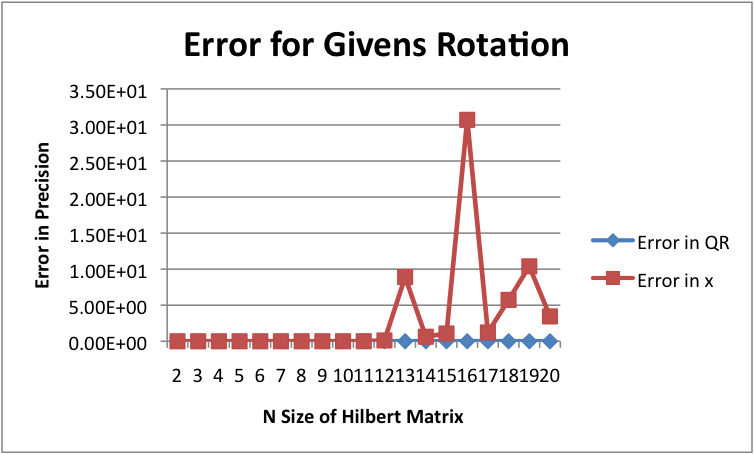
\includegraphics{givens.png}
  \caption{\label{givens}Error for Givens Rotation.}
\end{figure}

Again, like the Householder Reflection method, the Givens Rotation suffers odd
errors once it reaches the $13 \times 13$ Hilbert matrix.
And again, the problem arises because it is an ill-conditioned matrix.

\lstset{caption=Determining cond(R) for Givens}
\begin{lstlisting}[language=ruby]
for i in 2..20
  m = Matrix.hilbert(i)
  q,r = m.givens
  r_norm = r.power_method.abs
  r_inv_norm = r.inverse.power_method.abs
  puts "cond(N=#{i}): #{r_norm * r_inv_norm}"
end
\end{lstlisting}

Results were:

\begin{quote}
cond(N=2):  15.0000011125923
\\cond(N=3):  299.040144310689
\\cond(N=4):  6349.7651396892
\\cond(N=5):  138457.652248714
\\cond(N=6):  3063599.34834093
\\cond(N=7):  68420350.0720479
\\cond(N=8):  1537937656.71739
\\cond(N=9):  34733602598.1239
\\cond(N=10): 787216766308.864
\\cond(N=11): 17863296168299.8
\\cond(N=12): 4.05102981075616e+14
\\cond(N=13): 2.11135930217763e+16
\end{quote}

The Givens Rotation's $cond(R)$ ceases to calculate at $N=14$,
one dimension after the Householder Reflection.

\newpage
\section{Part Two}

%%
%% By: Jeff Drasher
%%

Clusterfuck.

\subsection{Jacobi Method}

Lots of stuff about Jacobi Method.

\subsection{Gauss-Seidel Method}

Lots of stuff about Gauss-Seidel Method.

\newpage
\section{Part Three}

%%
%% By: Mike Hirth
%%

The purpose of Part Three is to implement the Power Method in order to find the
largest eigenvalue of an $n \times n$ matrix, in particular a Leslie matrix that
models the population of a city. Using the Leslie matrix we can study the growth of populations by modeling the population distribution in future years and exploring the meaning of the Leslie matrix eigenvalue.

\subsection{Leslie Matrices}

Leslie Matrices are used to describe population growth in a city.
As shown in the problem, the first row of the matrix represents the per capita
average number of female offsprings of that age group, or the fecundity.
The following numbers in each column are the fractions of people surviving to the
next age class.
Each entry in the given population distribution matrix is the part of the
population in that age group, each group being of ten years (0-9,10-19, etc).
The first population distribution matrix given is for the year 2000 and is shown
later in listing 7.

The given Leslie Matrix of the city shown in Ruby is shown later on in listing 7 as well.

\subsection{Power Method}

The Power Method is used to calculate eigenvalues of $n \times n$ matrices.
In the class notes it was shown that after defining 

\[\vec{u}(n+1) = A\vec{u}(n)\]

it follows that

\[\lim_{n\to\infty} \frac{{\vec{w}} \cdot {\vec{u}(n+1)}}{ {\vec{w}} \cdot {\vec{u}(n)}} =\lambda\]

The following is an implementation of the Power Method in Ruby.
Its explanation is found in the solutions below.

\subsection{Implementation of the Power Method}
\lstset{caption=Power Method}
\begin{lstlisting}[language=ruby]
class Matrix
  def power_method
    a = self
    u_prev = Array.new(a.column_size) { 1 }
    w = Array.new(a.column_size) { |i| i == 0 ? 1 : 0 }
    lambda, innerProd1,innerProd2 = 0, 0, 0
    u_new_matrix = a * Vector[*u_prev].covector.transpose
    u_new_array = u_new_matrix.to_a
    u_new = []

    for i in 0...u_new_array.size
      u_new.push(u_new_array[i][0])
    end

    innerProd1 = innerProd1 + Vector[*w].inner_product(Vector[*u_new])
    innerProd2 = innerProd2 + Vector[*w].inner_product(Vector[*u_prev])
    lambda_prev = lambda
    lambda = (innerProd1/innerProd2).to_f
    u_prev = u_new
    u_new_matrix = a * Vector[*u_prev].covector.transpose
    u_new_array = u_new_matrix.to_a
    u_new = []

    for i in 0...u_new_array.size
      u_new.push(u_new_array[i][0])
    end

    while true
      innerProd1 = innerProd1 + Vector[*w].inner_product(Vector[*u_new])
      innerProd2 = innerProd2 + Vector[*w].inner_product(Vector[*u_prev])
      lambda_prev = lambda
      lambda = (innerProd1/innerProd2).to_f
      u_prev = u_new
      u_new_matrix = a * Vector[*u_prev].covector.transpose
      u_new_array = u_new_matrix.to_a
      u_new = []
      for i in 0...u_new_array.size
        u_new.push(u_new_array[i][0])
      end
      break if (lambda - lambda_prev).abs <= 0.00000001
    end
    return lambda
  end
end
\end{lstlisting}

\subsection{Answering the Question of Population Trends}

\subsubsection{Social Factors and Influences of the Leslie Matrix}

The original problem asks to interpret the data in the matrix and discuss the
social factors that influence those numbers.
The solution was derived from an analysis of the given Leslie matrix.

In the given Leslie matrix the survival rate in the different age groups and the
fecundity both vary.
The fecundity can be seen when analyzing the first row of the matrix.
In the age groups 0-9 and 50 and over, the average birth of females from that
age class is zero because women are not physically fertile.
In the ranges 10-19 and 20-29 the birth rate is low because women generally have
the most children in their thirties, which is apparent in the .9 per capita
average in that age group. 

Looking at the data in each of the columns of the matrix, the fraction of
surviving individuals varies due to several factors.
The number in each column represents the surviving fraction that makes it to the
next group.
Newborns of age 0-9 have a survival rate of .7 possibly due to infant deaths which
occur due to birth complications and medical problems.
The survival rates increase in the groups of 10-19 and 20-29, particularly
because individuals are the healthiest during this "prime" of their life.
The rate slowly decreases after 30-39 and over the next few age groups until it
drops .4 in the 70-79 age group in which health complications due to old age
cause more deaths.

\subsubsection{Projected Population Distributions}

In this implementation, the output is written to a file using the
\texttt{content} variable and the new matrices for the population distributions
are shown in the code.

\lstset{caption=Populations}
\begin{lstlisting}[language=ruby]
output = File.new("data3.txt", "w+")
content = ""

leslie = Matrix[[0,  1.2, 1.1,0.9,0.1 ,0  ,0   ,0   ,0],
                [0.7,0,   0,  0,  0,   0  ,0   ,0   ,0],
                [0,  0.85,0,  0,  0,   0  ,0   ,0   ,0],
                [0,  0,   0.9,0,  0,   0  ,0   ,0   ,0],
                [0,  0,   0,  0.9,0,   0  ,0   ,0   ,0],
                [0,  0,   0,  0,  0.88,0  ,0   ,0   ,0],
                [0,  0,   0,  0,  0,   0.8,0   ,0   ,0],
                [0,  0,   0,  0,  0,   0,  0.77,0   ,0],
                [0,  0,   0,  0,  0,   0,  0,   0.40,0]]

# largest eigenvalue of leslie

content << "largest lambda: #{leslie.power_method}\n"


# population distributions

x_0 = Matrix[[2.1], [1.9], [1.8], [2.1], [2.0], [1.7], [1.2], [0.9], [0.5]]
x_1 = leslie * x_0 #=> Matrix[[6.35], [1.47], [1.615], [1.62], [1.89], [1.76], [1.36], [0.924], [0.36]]
x_2 = leslie * x_1 #=> Matrix[[5.1875], [4.445], [1.2495], [1.4535], [1.458], [1.6632], [1.408], [1.0472], [0.3696]]
x_3 = leslie * x_2 #=> Matrix[[8.1624], [3.63125], [3.77825], [1.12455], [1.30815], [1.28304], [1.33056], [1.08416], [0.41888]]
x_4 = leslie * x_3 #=> Matrix[[9.656485], [5.71368], [3.0865625], [3.400425], [1.012095], [1.151172], [1.026432], [1.0245312], [0.433664]]
x_5 = leslie * x_4 #=> Matrix[[13.41322675], [6.7595395], [4.856628], [2.77790625], [3.0603825], [0.8906436], [0.9209376], [0.79035264], [0.40981248]]

# total populations

populations = [
               x_0.to_a.flatten.inject(&:+) * 10000,
               x_1.to_a.flatten.inject(&:+) * 10000,
               x_2.to_a.flatten.inject(&:+) * 10000,
               x_3.to_a.flatten.inject(&:+) * 10000,
               x_4.to_a.flatten.inject(&:+) * 10000,
               x_5.to_a.flatten.inject(&:+) * 10000
			   ]

content << "2010: #{populations[1]}
2020: #{populations[2]}
2030: #{populations[3]}
2040: #{populations[4]}
2050: #{populations[5]}
"

# percentage of population change

content << "2000 -> 2010: %.2f\%
2010 -> 2020: %.2f\%
2020 -> 2030: %.2f\%
2030 -> 2040: %.2f\%
2040 -> 2050: %.2f\%" % [((populations[1] - populations[0]) / populations[0] * 100),
                         ((populations[2] - populations[1]) / populations[1] * 100),
                         ((populations[3] - populations[2]) / populations[2] * 100),
                         ((populations[4] - populations[3]) / populations[3] * 100),
                         ((populations[5] - populations[4]) / populations[4] * 100)]
\end{lstlisting}

The next section requires a calculation of the population distribution, total
population, and fraction of change of the total population in 2010, 2020, 2030,
2040, and 2050. 

The approach to this problem was to use the Leslie Matrix Model and multiply the
Leslie Matrix by each previous population distribution, starting in 2010 and
using the given distribution for 2000.

The population distribution is shown in the code as matrices and written is

\vspace{11pt}

\begin{tabular}{l l}
$\vec{x}(1)$=&(6.35, 1.47, 1.615, 1.62, 1.89, 1.76, 1.36, 0.924, 0.36)($10^5$)\\
$\vec{x}(2)$=&(5.1875, 4.445, 1.2495, 1.4535, 1.458, 1.6632, 1.408, 1.0472, 0.3696)($10^5$)\\
$\vec{x}(2)$=&(8.1624, 3.63125, 3.77825, 1.12455, 1.30815, 1.28304, 1.33056, 1.08416, 0.41888)($10^5$)\\
$\vec{x}(4)$=&(9.656485, 5.71368, 3.0865625, 3.400425, 1.0121, 1.1512, 1.02643, 1.02453, 0.4337)($10^5$)\\
$\vec{x}(5)$=&(13.413227, 6.75954, 4.8566, 2.777906, 3.06038, 0.89064, 0.92094, 0.790353, 0.409812)($10^5$)
\end{tabular}

\vspace{11pt}

The total population of the city in question for each year was as follows:

\vspace{11pt}

\begin{tabular}{l l}
2010: & 173490.0 \\
2020: & 182815.0 \\
2030: & 221212.4 \\
2040: & 265050.467 \\
2050: & 338794.2932
\end{tabular}

\vspace{11pt}

With the fractional change of the total population:

\vspace{11pt}

\begin{tabular}{l l}
2000 $\to$ 2010: & 22.18\% \\
2010 $\to$ 2020: & 5.37\% \\
2020 $\to$ 2030: & 21.00\% \\
2030 $\to$ 2040: & 19.82\% \\
2040 $\to$ 2050: & 27.82\%
\end{tabular}

\vspace{11pt}

By implementing the formula given in the problem

\[\vec{x}(k + 1) = A\vec{x}(k)\]
 
where $k = 0,1,2,3,4,5$ and $\vec{x}(0)$ is the given
population distribution, the population distribution could be calculated for
each decade increase.
This, more simply put, is a multiplication of the Leslie matrix with the
previous population distribution. This is seen in the code as
\texttt{x\_1 = leslie * x\_0} where \texttt{x\_0} is the $\vec{x}(0)$ population
distribution. The next decades are calculated in the same manner.
In order to find the total population of one year, a simple summation of the
elements of each of the population distribution matrices (multiplied by $10^5$)
shown in the code as \texttt{population} gives the total population.
The percent increase of the population was calculated by taking the difference
in total population divided by the previous population,
for each decade as seen in the last portion of the code in listing 7. 

\subsubsection{Obtaining the Eigenvalue and its Meaning}

In order to evaluate these populations it was required to write a program
implementing the Power method to calculate the largest eigenvalue of an
$n \times n$ matrix where the method stops after 8 digits of accuracy.
The program could be used to calculate the largest eigenvalue of the given
Leslie matrix.

The bulk of this problem was in developing a Power method algorithm in Ruby that
took in an $n \times n$ matrix that iterated until 8 digit decimal precision was
achieved.
After testing to see if the program returned correct eigenvalues for any square
matrix, it was passed the Leslie matrix in order to find the largest eigenvalue.

After running the program using the Leslie matrix, the method returns the
eigenvalue 1.28865626235758.

Implementing the power method in Ruby only required the creation of one method
because of some shared coding with part 1 including the
\texttt{Vector\#inner\_product} method to calculate the dot product,
used in part of the algorithm.
The general formula for the power method can be found in the web notes by Laszlo Erdos
for \textit{Linear Algebra: Numerical Methods in Numerical Computation of Eigenvalues}(p 62).


\[\lim_{n\to\infty} \frac{{\vec{w}} \cdot {\vec{u}(n+1)}}{ {\vec{w}} \cdot {\vec{u}(n)}} =\lambda\]

where $\vec{w}$ and $\vec{u}_0$ are randomly chosen nonzero vectors.
As shown in the declarations of \texttt{u\_prev} and \texttt{w} in the power
method program implemented uses a $\vec{w}$ vector of $[1,0,0 ... ,0_n]^t$
and a $\vec{u}_0$ vector of $[1,1,1 ... ,1_n]^t$ both with the number of entries
equal to $n$ of the $n \times n$ Leslie matrix.
These are the vectors we used in class to compute eigenvalues with the Power
Method but they could be any vectors as long as they are not zero.
The coding of the algorithm for the actual iterations of the method can be seen
in the while loop.
There are two general parts to calculating the eigenvalue.
First, $\vec{u}_1$ is calculated and later $\vec{u}_{(n+1)}$ with the same code
but over many iterations in the while loop, represented in the code, after
certain conversions, as \texttt{u\_new}.
This is modeled by $\vec{u}_{(n+1)} = A\vec{u}_{(n)}$ on page 62 of the web
notes by Erdos, where in the code \texttt{u\_new} is $\vec{u}_{(n+1)}$,
\texttt{u\_prev} is $\vec{u}_n$ and \texttt{a} is $A$, the given matrix.

The second part involves the eigenvalue calculated using the inner products
according to the limit exampled earlier.
The code is first implemented when using \texttt{innerProd1} and
\texttt{innerProd2} and later on over multiple iterations, where \texttt{lambda}
is the approximated eigenvalue and \texttt{lambda\_prev} is saved for precision
calculation.
The break statement terminates the loop after the difference in lambdas is less
than $10^{-8}$, guaranteeing that precision.
The first iteration does not have a lambda to compare so it occurs outside and
before the loop, creating some repetition of code.
When converting matrices to arrays in order to multiply the inner product we encounter a small problem in Ruby.
When using the \texttt{Matrix\#.to\_a} the given matrix is converted to an
array of arrays containing numbers instead of just an array of numbers.
To take care of this, a new array is created and filled with the elements of
the old array shown as \texttt{u\_new.push(u\_new\_array[i][0])}.
In the code the first calculation of $\vec{u}_{(n+1)}$ is \texttt{u\_new\_matrix}
and in Ruby is of the type \texttt{Matrix}.
The array conversion is denoted as \texttt{u\_new\_array} and finally the array
of numbers which can actually be used is \texttt{u\_new}.
Once lambda is calculated as a float point of precision to 8 decimals it is
returned by \texttt{Matrix\#power\_method}.

The next part of the problem asked to analyze the eigenvalue obtained for the
Leslie matrix and discuss what this means about the growth of the population in
the long run.

Obtaining the eigenvalue of 1.28865626 reveals the eventual behavior of the
population of the given city.
The eigenvalue is greater than 1 which means the population will grow.
If it was less than 1, the population would over time become extinct and if
it was equal to 1 then the population would remain the same, with equal birth and death.
This can be shown using the theorem covered in chapter 4 of Erdos's notes (p 49):

\begin{quote}
Theoreom 4.1

For a square matrix $A$,
$||A^k|| \to 0$ if and only if, all eigenvalues of $A$ satisfy $|\lambda| < 1$

When looking at the iterative model given in the question 

\[\vec{x}(k) = A^k \vec{x}(0)\]

it is possible to see that a norm that converges to zero with a large enough k would eventually give a population of zero when multiplied by the distribution vector.
This would happen if the largest eigenvalue was less than 1, and it can be drawn that because our eigenvalue computed for
the Leslie matrix is greater than 1 the population must grow, getting closer to that rate as k gets larger.

Therefore we arrive at the equation

\[\vec{x}(n+1) = \lambda\vec{x}(n)\]

for large values of $n$, where $\lambda$ is the dominant or largest eigenvalue.
\end{quote}

This shows that as n gets larger $\vec{x}(n+1)$ is a scalar multiple of $\vec{x}(n)$ and if that scalar,
the computed eigenvalue, is positive the population will eventually grow by that growth rate,
as shown in our given case of the population of a city.

\subsubsection{Supposing a Change in Birth Rate}

In this implementation, the output is written to a file using the \texttt{content} variable

\lstset{caption=Populations}
\begin{lstlisting}[language=ruby]
leslie = Matrix[[0,  0.6, 1.1,0.9,0.1 ,0  ,0   ,0   ,0],
                [0.7,0,   0,  0,  0,   0  ,0   ,0   ,0],
                [0,  0.85,0,  0,  0,   0  ,0   ,0   ,0],
                [0,  0,   0.9,0,  0,   0  ,0   ,0   ,0],
                [0,  0,   0,  0.9,0,   0  ,0   ,0   ,0],
                [0,  0,   0,  0,  0.88,0  ,0   ,0   ,0],
                [0,  0,   0,  0,  0,   0.8,0   ,0   ,0],
                [0,  0,   0,  0,  0,   0,  0.77,0   ,0],
                [0,  0,   0,  0,  0,   0,  0,   0.40,0]]

x_3new = leslie * x_2
x_4new = leslie * x_3new
x_5new = leslie * x_4new

populations_new = [
                   x_2.to_a.flatten.inject(&:+) * 10000,
                   x_3new.to_a.flatten.inject(&:+) * 10000,
                   x_4new.to_a.flatten.inject(&:+) * 10000,
                   x_5new.to_a.flatten.inject(&:+) * 10000
                  ]

content << "\n\nWith 2020's second set modified.
"

content <<  "2020: #{populations_new[0]}
2030: #{populations_new[1]}
2040: #{populations_new[2]}
2050: #{populations_new[3]}
"
content << "largest lambda: #{leslie.power_method}\n"

content << "2020 -> 2030: %.2f\%
2030 -> 2040: %.2f\%
2040 -> 2050: %.2f\%" % [((populations_new[1] - populations_new[0]) / populations_new[0] * 100),
                         ((populations_new[2] - populations_new[1]) / populations_new[1] * 100),
                         ((populations_new[3] - populations_new[2]) / populations_new[2] * 100)]

output.write(content)
\end{lstlisting}

The problem asks to decrease the birth rate of the second age group by half in 2020
and then predict the population for 2030, 2040 and 2050, discussing again the meaning
of the eigenvalue for this new matrix over a long period of time.

This was approached by changing the original Leslie matrix to reflect the new change
in birth rate and then applying the previous method of calculating using the total populations
and fractional change for the years of 2030, 2040, and 2050. 

The newly computed eigenvalue is 1.16790279. The new populations of the following years are:

\vspace{11pt}

\begin{tabular}{l l}
2020: & 182815.0 \\
2030: & 194542.4 \\
2040: & 224593.967 \\
2050: & 262190.9132
\end{tabular}

\vspace{11pt}

and the percentage of change in populations are

\vspace{11pt}

\begin{tabular}{l l}
2020 $\to$ 2030: & 6.41\% \\
2030 $\to$ 2040: & 15.45\% \\
2040 $\to$ 2050: & 16.74\%
\end{tabular}

\vspace{11pt}

These values were arrived at by first altering the Leslie matrix as seen above, where
the birth rate of the second age group, which was previous at 1.2 was decreased to 0.6.
This birth rate changes in 2020 so the population distribution in 2010 and 2020 remains the same as
presented in the data.
In calculating the distribution in 2030, the calculation used before still applies but includes the
new Leslie matrix.
The population distribution in 2030 is equal to the new Leslie matrix times the population
distribution in 2020.
In Ruby this looks like \texttt{x\_3new = leslie * x\_2} and the code following it,
where \texttt{x\_3new, x\_4new, x\_5new} are all of the new distribution matrices.
Once these are calculated the total populations can be found by using the same method earlier,
which was to add each of the numbers in the population distribution in \texttt{populations\_new}.
Finding the percent change was also the same as previously done. 

The eigenvalue is computed by using the Power Method on the new Leslie matrix, using a simple call to the method \texttt{leslie.power\_method}

This eigenvalue is still a positive number greater than 1, showing a population that will still grow positively and eventually
level off at a factor of 1.167902791647756 for the new birth rate, which is somewhat lower than the previous rate.
The population totals show the growing populations diminish due to the halved birthrate of the second age group in 2020. By
2050 where the population would have been 338794.2932 it is now 262190.9132.
However, in the long run the population will not diminish because it's dominant eigenvalue is still greater than 1.

\end{document}